\section{Commercial Impedance Measurement} \label{sec:CommercialImpedanceMeasurement}
Most of the major manufacturers of test equipment, such as Keysight Technologies, Rohde \& Schwarz, Tektronix and others produce a range of instruments for characterizing passive components. This section will review a few of these to research their capabilities, to indicate what a user might want and need.

LCR meters typically come in two different form factors, one is a handheld device, much like a regular multimeter, while the other is a benchtop instrument. The handheld LCR meters, like the Keysight U1733C\cite{KeysightU1733C}, shown in figure \ref{fig:2_2_U1733C}.
\begin{figure}[H]
    \centering
    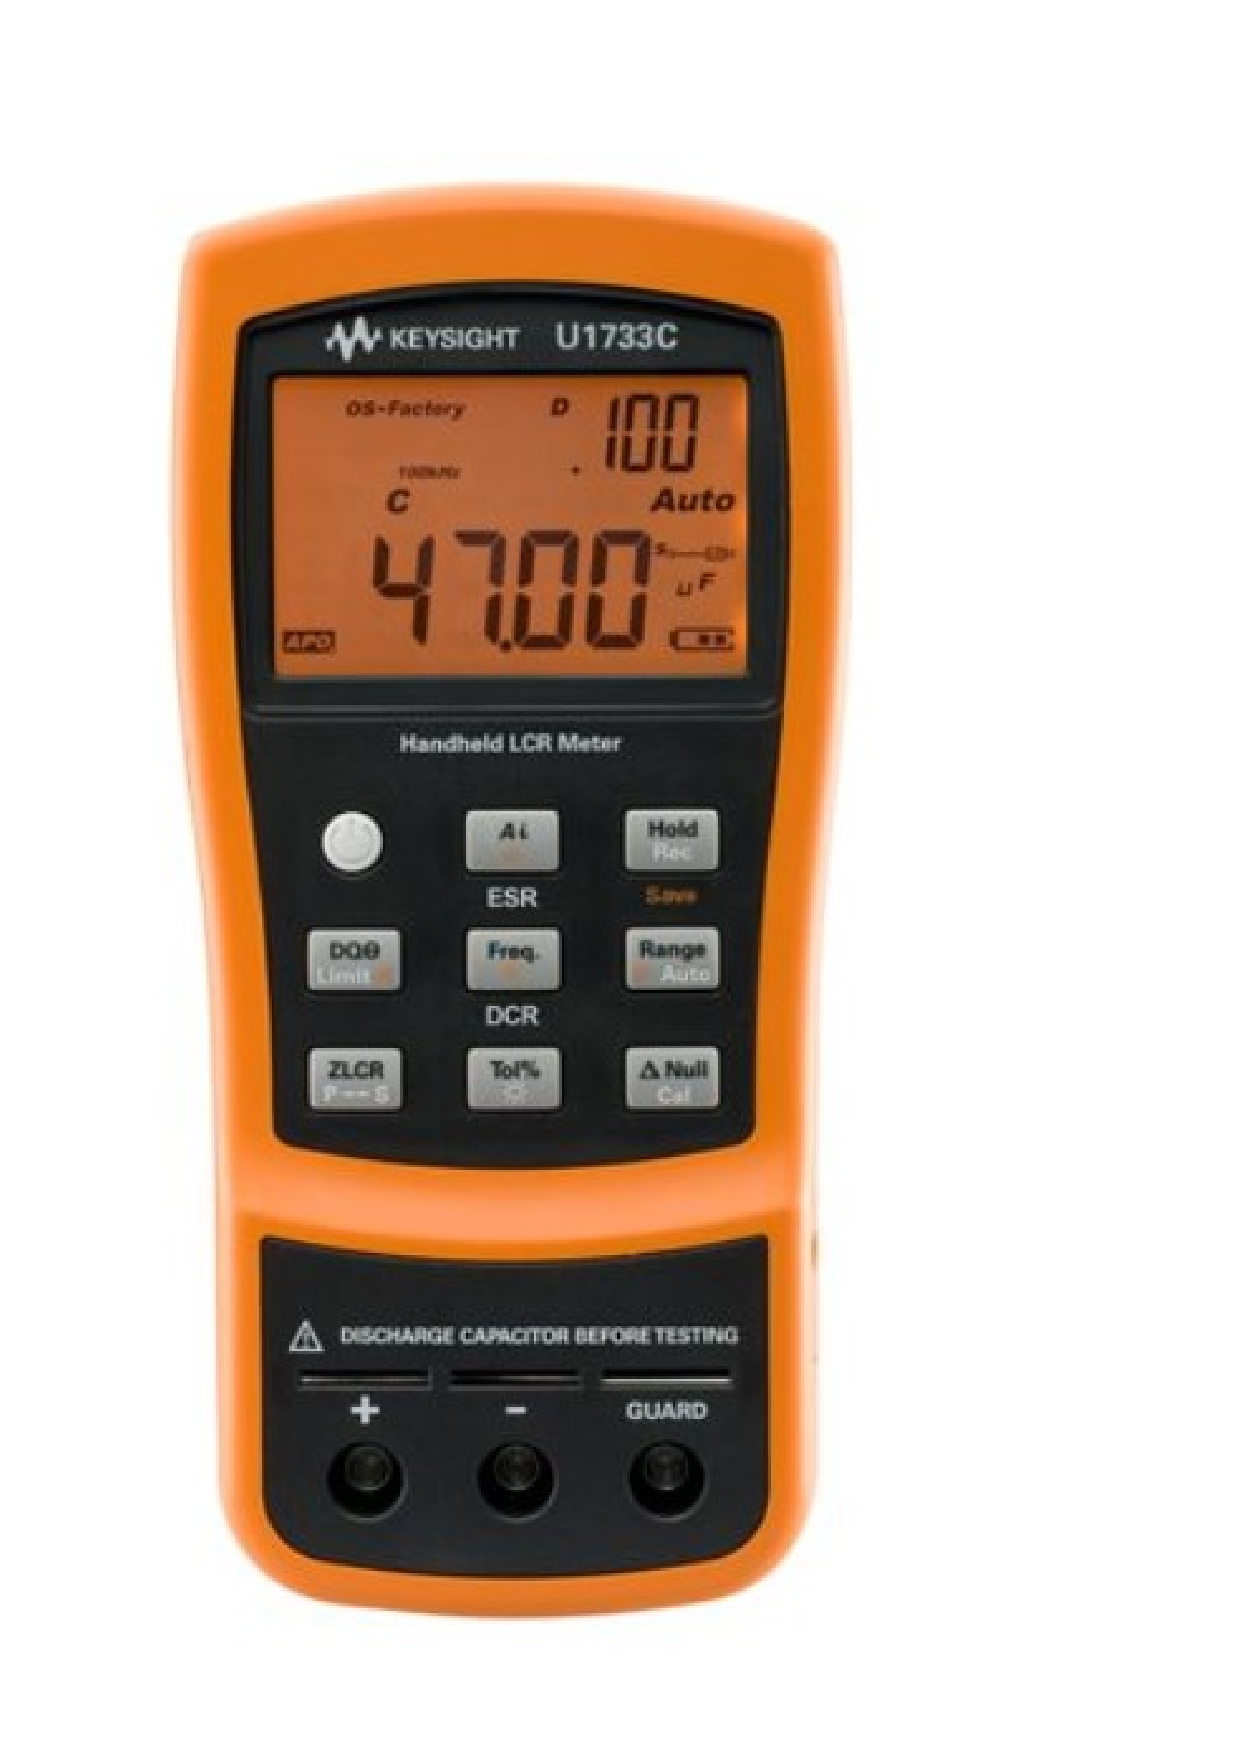
\includegraphics[clip, trim=0 50 0 50, width=0.5\textwidth]{Sections/2_ProblemAnalysis/FIgures/KeysightU1733C.pdf}
    \caption{A handheld Keysight U1733C LCR meter.\cite{KeysightU1733C}}
    \label{fig:2_2_U1733C}
\end{figure}
The U1733C shown on \ref{fig:2_2_U1733C} is meant for troubleshooting and repair work and not for engineering use, while it is affordable at about 550€, it has limited capabilities. It can measure all the basic parameters such as capacitance, inductance, ESR and display all the derived quantities like dissipation and quality factor numerically, however it can only take these measurements at a pre-determined set of test frequencies in the range \SI[]{100}{\hertz} to \SI[]{100}{\kilo\hertz} with measurement accuracy weaning off in both ends of the frequency range as shown on figure \ref{fig:2_2_U1733CCapAccurancy}.

\begin{figure}[H]
    \centering
    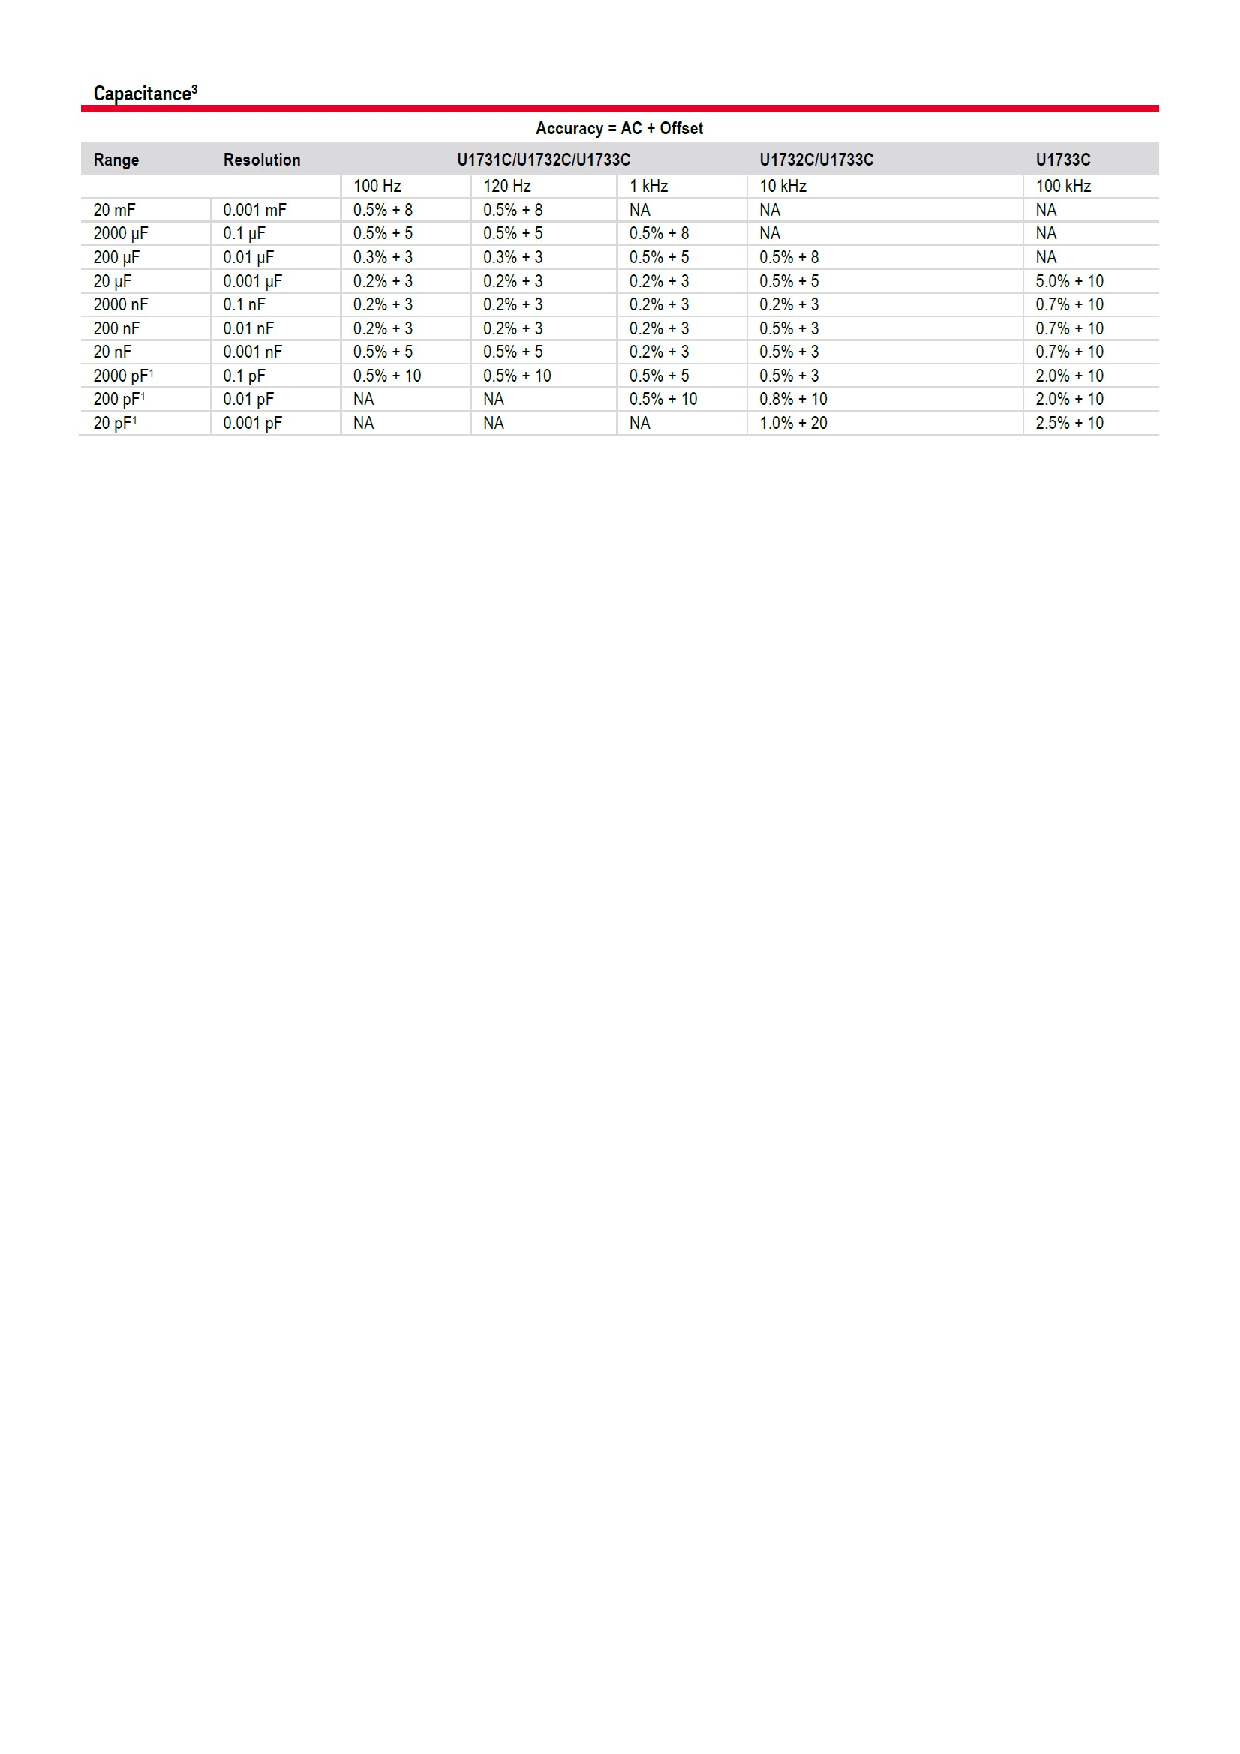
\includegraphics[clip, trim=0 630 0 0, width=1\textwidth]{Sections/2_ProblemAnalysis/FIgures/U1733CAccuracyDatasheet.pdf}
    \caption{A snapshop from the Keysight U1733C datasheet listing the accuracy of capacitance measurements.\cite{KeysightU1733CDatasheet}. Measurements for inductance, resistance and so on show a similar pattern.}
    \label{fig:2_2_U1733CCapAccurancy}
\end{figure}

The U1733C datasheet has similar charts for other measurements, but they follow a similar pattern of accuracy as capacitance where it becomes clear that the accuracy is worse in the higher ends of the range. The accuracy is listed as a $\%$ of range $ + n\cdot resolution$, so a measurement in the \SI[]{20}{\micro\farad} range will have an accuracy of $\pm \SI[]{1}{\micro\farad} + \SI[]{10}{\nano\farad} = \SIQ{1.01}{\micro\farad}$ at \SIQ{100}{\kilo\hertz}.

Rohde \& Schwarz has a benchtop line of LCR meters called the LCX line \cite{RSLCXLCRMeters}. These have tighter specifications for accuracy, a greater range and a more diverse set of displaying the measurements. They also come with a significantly higher price tag at 15000€ for a 500kHz bandwidth version. This LCR meter is shown on figure \ref{fig:2_2_RSLCX}.
\begin{figure}[H]
    \centering
    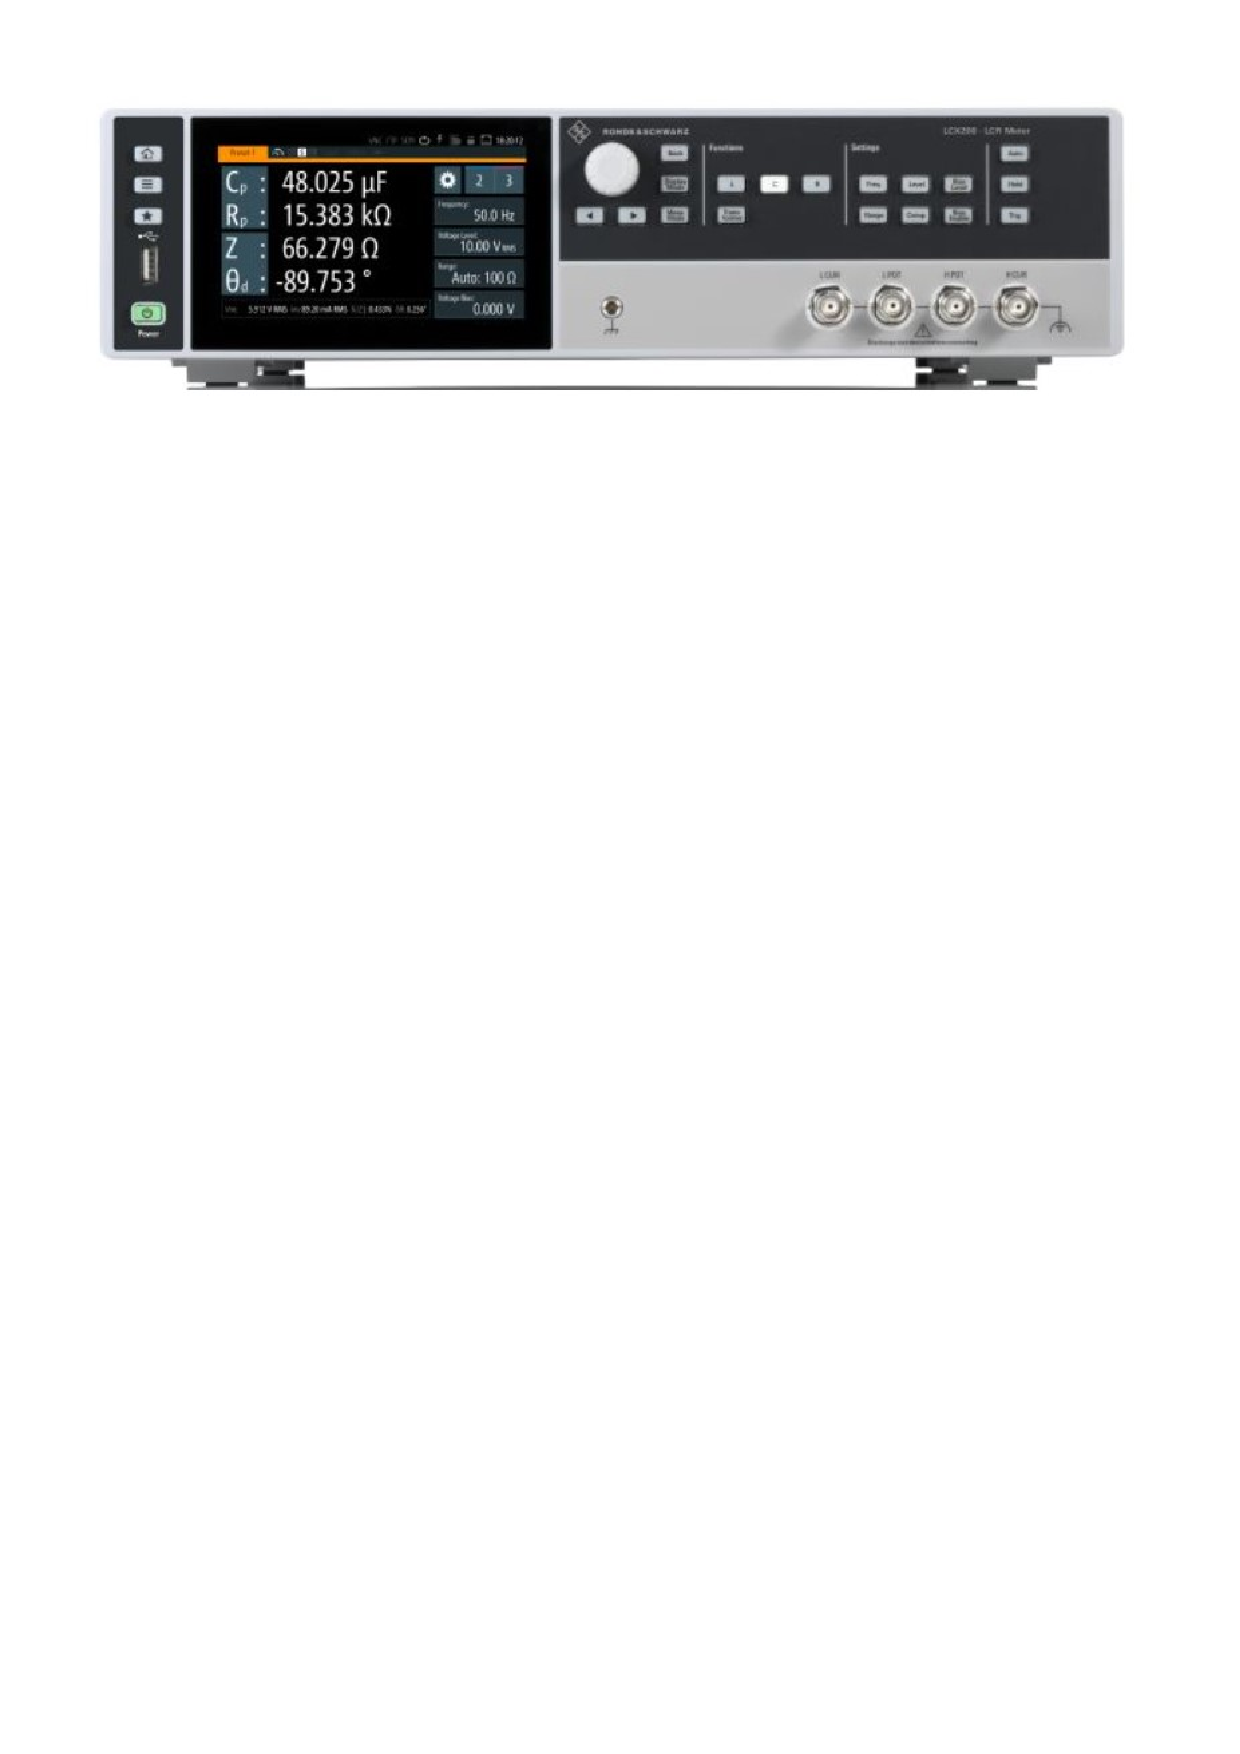
\includegraphics[clip, trim=0 630 0 50, width=1\textwidth]{Sections/2_ProblemAnalysis/FIgures/RSLCXLCR.pdf}
    \caption{A Rohde \& Schwarz LCX LCR meter featured a significantly greater bandwidth when compared to the U1733C, 4-wire kelvin measurements and greater ability to display the measurements.\cite{RSLCXLCRMeters}}
    \label{fig:2_2_RSLCX}
\end{figure}

The Rohde \& Schwarz LCX LCR meter is using kelvin bridge (4-wire) measurements.  This feature is often seen on higher end test equipment in order for the instrument to compensate for the parasitics introduced by the test instruments own test leads. The instrument can be triggered to take measurements externally and be controlled remotely over various network interfaces. The meter also has a sweep function in order to measure the impedance of the DUT over a series of frequency values and can display all the measurements numerically of graphically. Unlike the U1733C this meter is intended for electronic development purposes.

The Wayne-Kerr 6500B\cite{WayneKerr6500} series is a high-end impedance analyzer for demanding applications. The industry differentiates between \textit{LCR meters} and \textit{Impedance analyzers}. An LCR meter will display it's single point measurements numerically, while an impedance analyzer can do the same but is meant specifically for frequency sweeps and displaying the measurements on graphs. In other words, an impedance analyzer is a more advanced LCR meter. The Wayne-Kerr 6500B is shown on figure \ref{fig:2_2_WayneKerr6500B}. 
\begin{figure}[H]
    \centering
    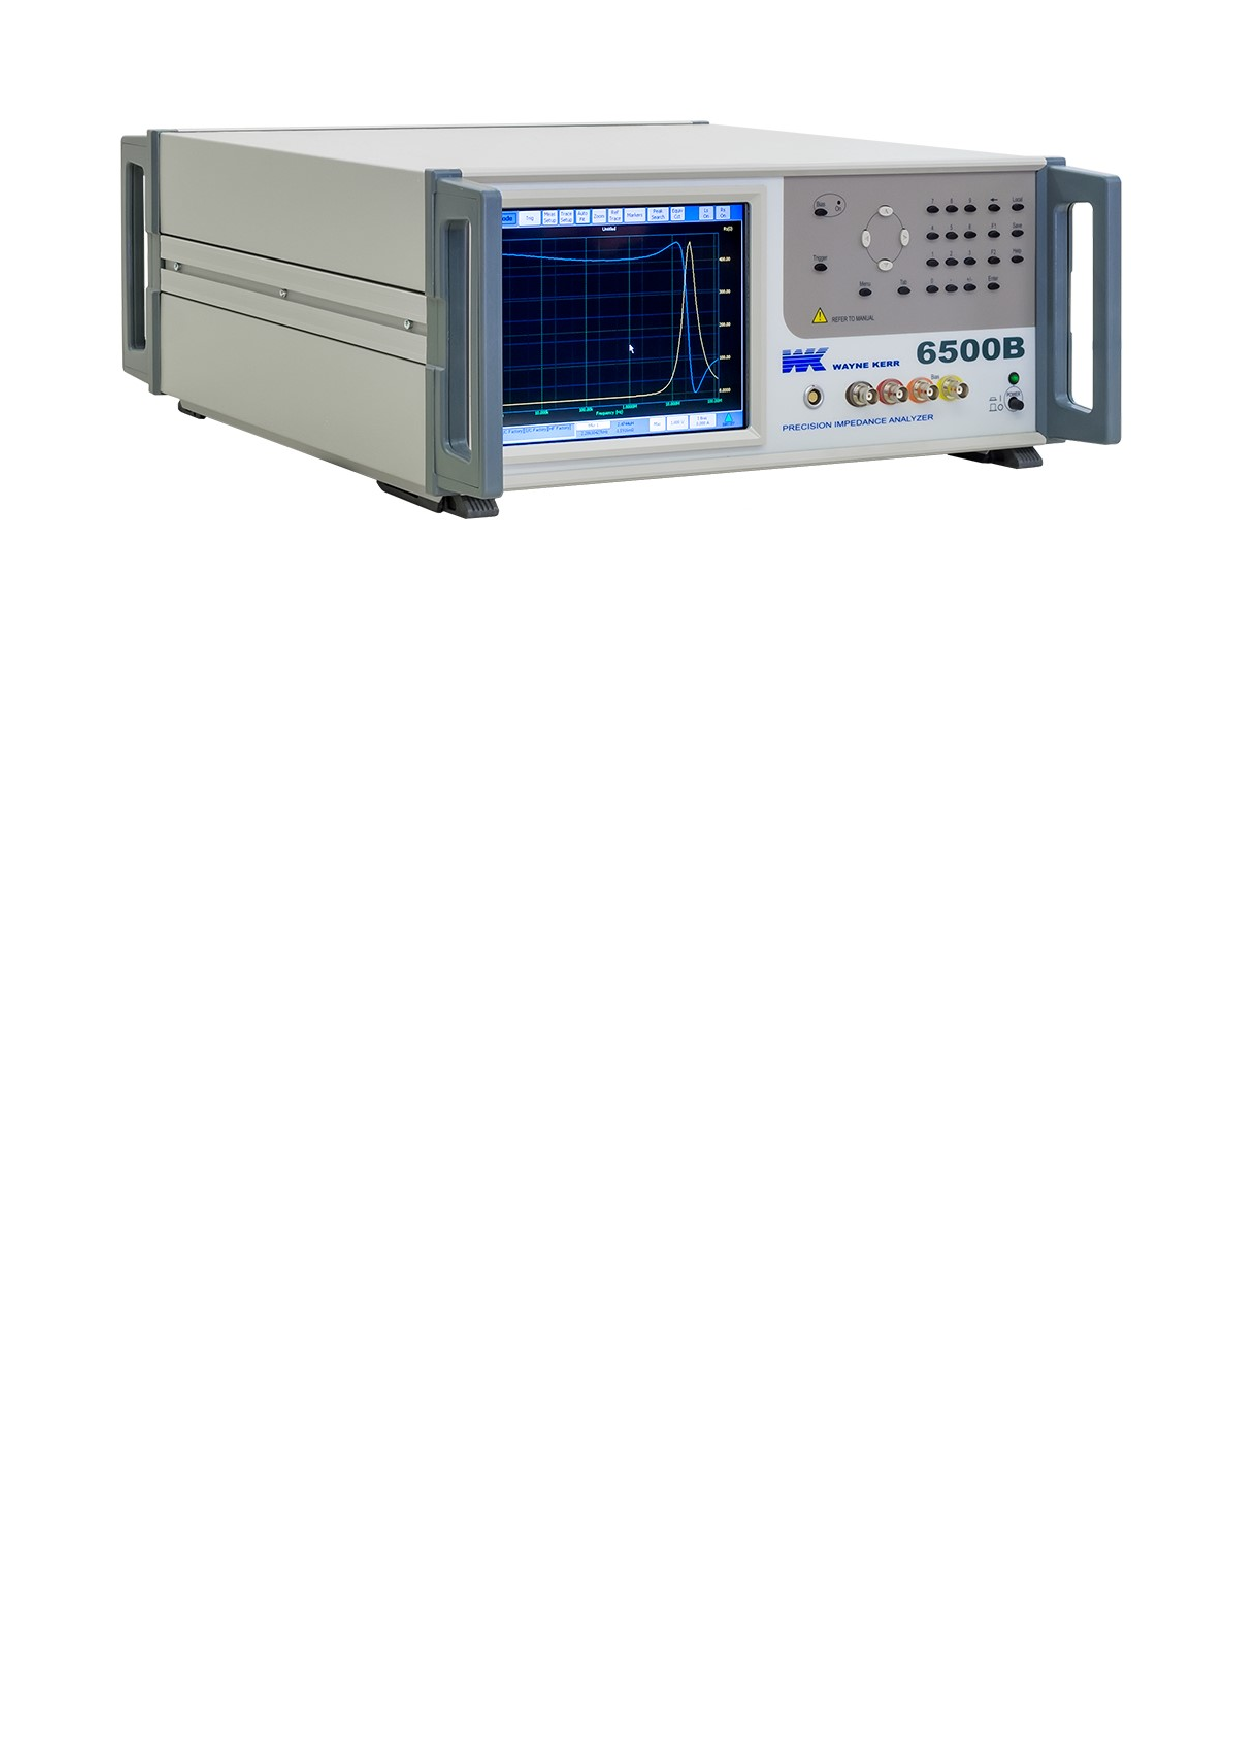
\includegraphics[clip, trim=0 550 0 50, width=1\textwidth]{Sections/2_ProblemAnalysis/FIgures/WayneKerrImpedanceAnalyzer.pdf}
    \caption{A Wayne-Kerr 6500B impedance analyzer. Note how it displays it's measurements graphically.}
    \label{fig:2_2_WayneKerr6500B}
\end{figure}
This impedance analyzer has a test frequency range of \SI[]{20}{\hertz} to \SI[]{120}{\mega\hertz} and has a test frequency resolution of \SI[]{100}{\micro\hertz} and Wayne-Kerr guarantees an accuracy of L, C and R measurements of $\pm 0.05$ \% across the entire frequency range putting this instrument in a different league from the ones previously shown. This impedance analyzer has adjustable DC bias as well, so bias stability can be measured as well. The impedance analyzer can display it's measurements on regular plots but can also show them in polar, or complex, form much like a network analyzer. The price of this instrument is listed as \textit{request quote} putting it far out of reach of even most smaller companies.


